\chapter{Narukvica}
\label{pog:bracelet}
Svrha narukvice je prikupljanje fizioloških signala korisnika i njihovo slanje na obradu na središnjem uređaju putem bežičnog komunikacijskog sučelja. Fiziološki signali koji će se promatrati su brzina otkucaja srca putem fotopletizmografskog senzora (PPG) i impedancija kože, odnosno elektrodermalna aktivnost.

Što se tiče zahtjeva na napajanje narukvice, zahtjevi su slični kao i kod središnjeg uređaja, uz nižu potrošnju. Prilikom projektiranja narukvice iskorišteno je iskustvo stečeno projektiranjem i ispitivanjem pločice središnjeg uređaja tako da su u dizajnu narukvice popravljeni nedostaci inicijalnog dizajna vezanog uz napajanje kako je implementirano na pločici središnjeg uređaja. S obzirom na ograničenje na veličinu pločice za narukvicu, za razliku od implementacije središnjeg uređaja, ovdje nisu postavljeni dodatni kratkospojnici i ispitne točke za lakše testiranje, s obzirom da je sličan dizajn već ranije ispitan tijekom uhodavanja središnjeg uređaja.

\section{Bežična komunikacija}
Za ostvarenje bežične komunikacije koristi se modul ESP32-C3-WROOM-02-N4, koji omogućuje komunikaciju putem Bluetooth i Wi-Fi protokola. Električna shema dijela za bežičnu komunikaciju na narukvici (slika \ref{slk:BR_WIRELESS}) slična je implementaciji na pločici središnjeg uređaja (slika \ref{slk:WIFI}), uz razliku da ovdje nema kratkospojnika, uz dodatak signala za upravljanje I\textsubscript{2}C sučeljem i korištenje analogno-digitalnog pretvornika za mjerenje impedancije kože. Postoji još i promjena u odnosu na implementaciju na središnjem uređaju, a odnosi se na programiranje putem UART-a. S obzirom na uočene probleme u programiranju pločice središnjeg uređaja, dodani su signali DTR i CTS kako bi se BOOT i EN stezaljke ESP mikrokontrolera mogle programski upravljati.
\begin{sidewaysfigure}[htbp]
    \centering
    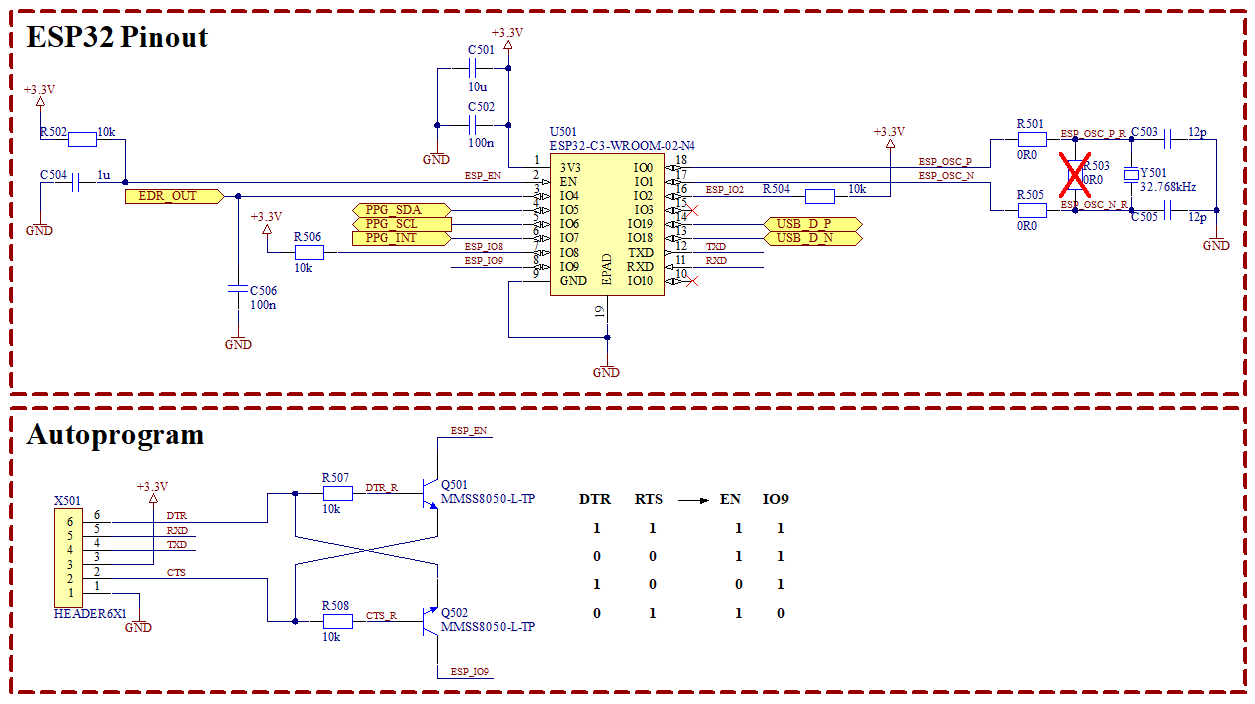
\includegraphics[width=1\textwidth]{Figures/BR_WIRELESS.png}
    \caption{Električna shema bežične komunikacije narukvice}
    \label{slk:BR_WIRELESS}
\end{sidewaysfigure}

\newpage
\section{Fotopletizmografski senzor}

Za mjerenje brzine otkucaja srca koristi se PPG senzor MAX30101 tvrtke Analog Devices (slika \ref{slk:MAX30101}). Ovaj senzor sadrži crvenu, zelenu i infracrvenu svjetleću diodu te fotosenzor, upravljačko sklopovlje za diode, a komunicira putem I\textsuperscript{2}C sučelja. Kao što je vidljivo na električnoj shemi na slici \ref{slk:PPG}, ovaj senzor je jednostavan za implementaciju uz svega par priteznih otpornika i blokadnih kondenzatora. Određenu složenost unosi potreba za napajanjem od 5 V, koje je potrebno jer je pad napona na zelenoj svjetlećoj diodi prema specifikaciji 3,3 V.
\begin{figure}[htb]
    \centering
    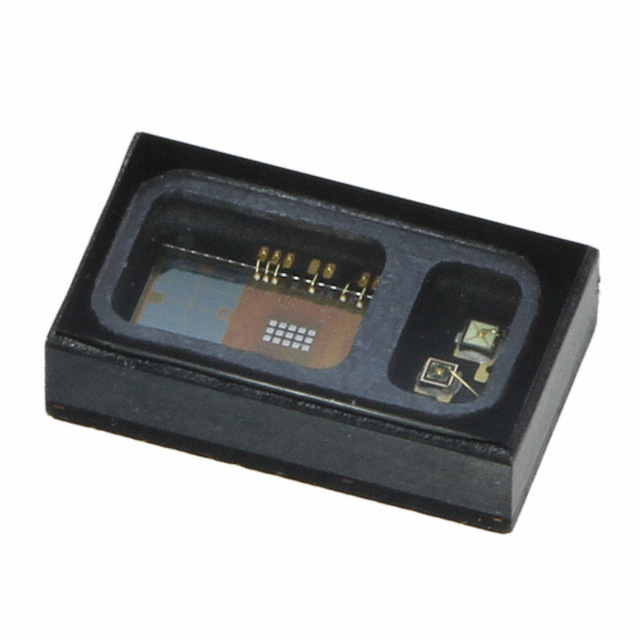
\includegraphics[width=6 cm]{Figures/MAX30101.JPG}
    \caption{MAX30101 PPG senzor}
    \label{slk:MAX30101}
\end{figure}
\begin{figure}[htb]
    \centering
    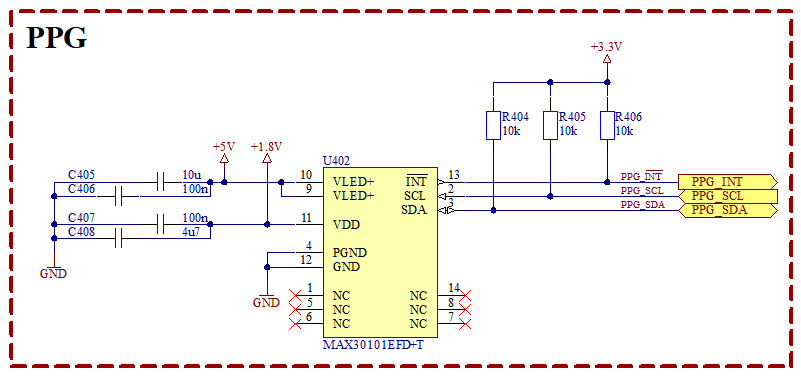
\includegraphics[width=\textwidth]{Figures/PPG.png}
    \caption{Električna shema PPG senzora}
    \label{slk:PPG}
\end{figure}

\section{Mjerenje impedancije kože}
Impedancija kože mjeri se pomoću instrumentacijskog pojačala. Električna shema mjernog kruga prikazana je na slici \ref{slk:EDR}. Odabrano je instrumentacijsko pojačalo AD8226 tvrtke Analog Devices zbog svog velikog ulaznog otpora, niskog šuma i dobrog potiskivanja zajedničkih smetnji \cite{ad:ad8226}. Napajanje pojačala filtrirano je pasivnom mrežom kako ne bi došlo do smetnji od digitalnog dijela sklopovlja.
\begin{figure}[htb]
    \centering
    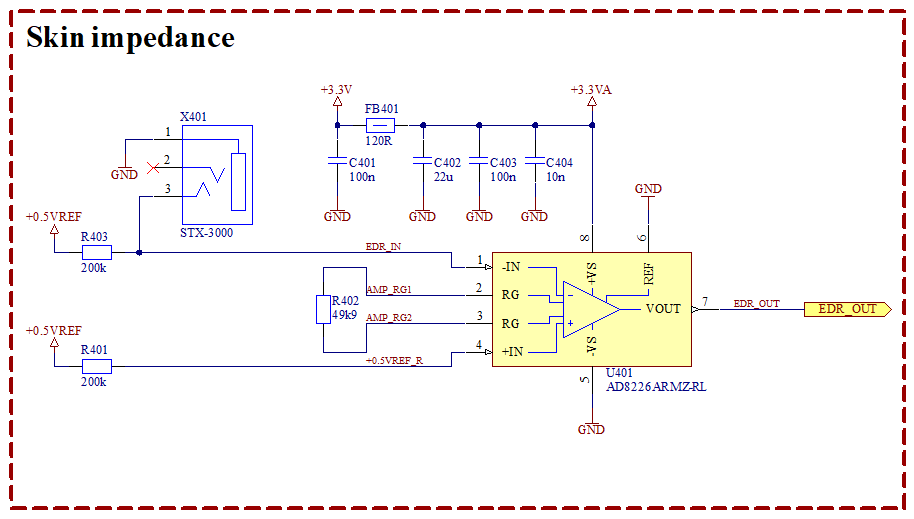
\includegraphics[width=\textwidth]{Figures/EDR.png}
    \caption{Električna shema mjernog kruga za impedanciju kože}
    \label{slk:EDR}
\end{figure}
Za mjerenje impedancije koristi se referentni napon od 0,5 V, a postupak mjerenja temelji se na mjerenju napona na naponskom djelilu na stezaljci -IN pojačala. Koža predstavlja donji otpornik u naponskom djelilu te se razlika između tog napona i referentnog napona pojačava:
\begin{equation} \label{eq:EDR}
    U_{IZ}=A\cdot U_{REF}\cdot \frac{R_{403}}{R_{403}+R_{skin}}
\end{equation}
Impedancija kože mjeri se u stotinama kilooma (maksimalno cca. $250\textrm{ k}\Omega$ \cite{rskin}), tako da je vrijednost gornjeg otpornika $200\textrm{ k}\Omega$. Pojačanje iznosi 2 i namješta se putem otpornika R402.

U svrhu lakšeg prototipiranja koristile su se samoljepljive elektrode (slika \ref{slk:ELECTRODE}) koje se montiraju na kabel prikazan na slici \ref{slk:CABLE}. 
\begin{figure}[htb]
    \centering
    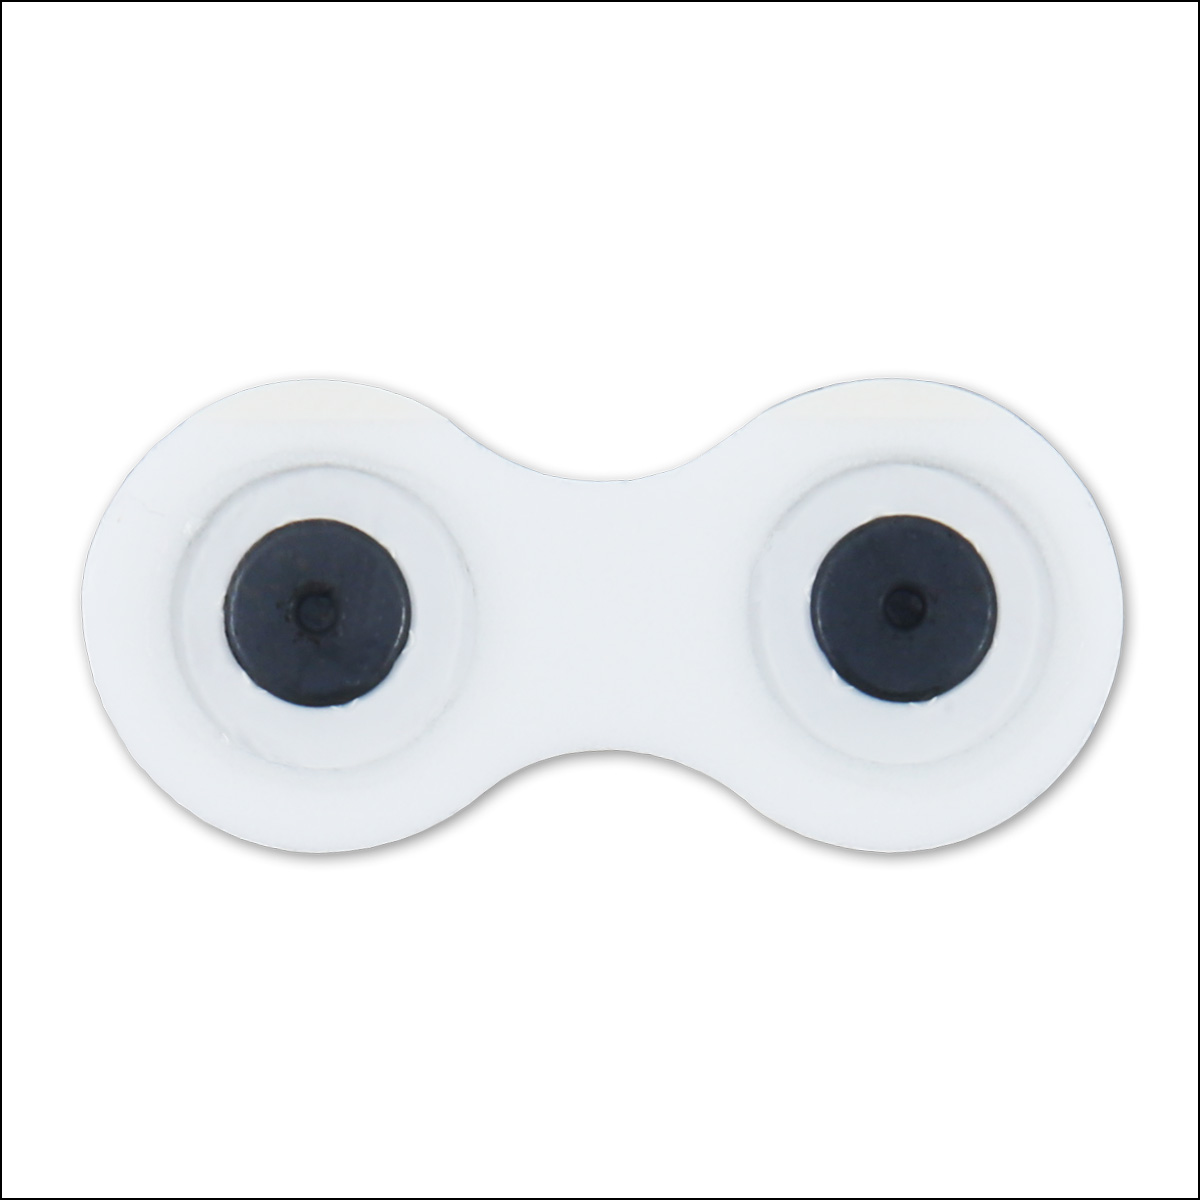
\includegraphics[width=6 cm]{Figures/ELECTRODE-BOTTOM.jpg}
    \caption{Samoljepljiva elektroda}
    \label{slk:ELECTRODE}
\end{figure}
\begin{figure}
    \centering
    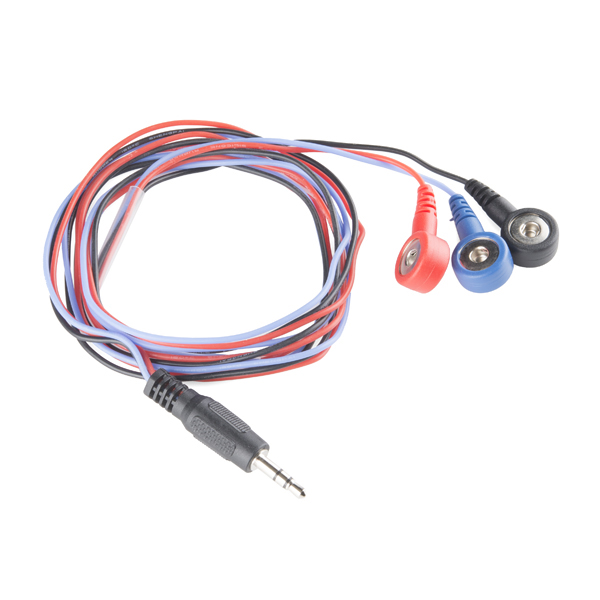
\includegraphics[width=6 cm]{Figures/CABLE.jpg}
    \caption{Kabel za elektrode}
    \label{slk:CABLE}
\end{figure}
Ovaj kabel se spaja na narukvicu putem 3,5 mm audio priključka.

\section{Napajanje}
\subsection{Proračun potrošnje}

Proračun potrošnje za narukvicu bio je znatno jednostavniji od proračuna za središnji uređaj. U slučaju ove pločice najveći potrošač je i dalje sustav za bežičnu komunikaciju, koji je i ujedno jedini potrošač na 3,3 V jer je potrošnja instrumentacijskog pojačala zanemarivo niska, maksimalno 20 $\mu\textrm{A}$ \cite{ad:ad8226}. Za potrošnju sustava bežične komunikacije uzima se vrijednost prikazana u tablici \ref{tab:MB3V3}. Na napajanju od 5 V jedini potrošač je PPG senzor i njegova potrošnja u najgorem slučaju iznosi 50 mA, a na napajanju od 1,8 V senzor troši maksimalno 1,1 mA \cite{ad:max30101}.

\subsection{Napajanja od 3,3 V i 1,8 V}
\label{subsec:BR_VDD}
Električne sheme napajanja od 3,3 V i 1,8 V prikazane su na slici \ref{slk:BR_VDD}. U oba slučaja koristi se LDO AP2112K proizvođača Diodes Incorporated. Ovaj LDO je odabran radi svoje male veličine u SOT-25 kućištu s obzirom na ograničenje veličine tiskane pločice.
\begin{figure}[htb]
    \centering
    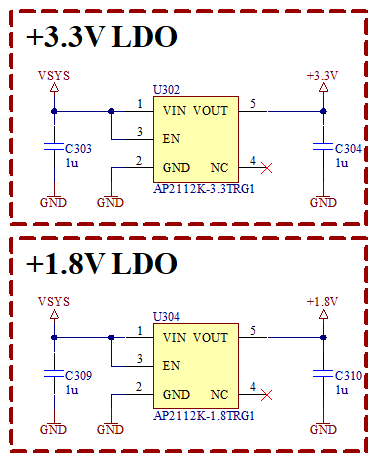
\includegraphics[width=6 cm]{Figures/BR_VDD.png}
    \caption{Napajanje od 3,3 V i 1,8 V za narukvicu}
    \label{slk:BR_VDD}
\end{figure}

\subsection{Referentni napon}

Električna shema izvora referentnog napona prikazana je na slici \ref{slk:BR_VREF}. Koristi se izvor referentnog napona ADR130 tvrtke Analog Devices. Iznos referentnog napona se može namjestiti na 1 V ili 0,5 V, a veličina kućišta je ista kao i kod linearnih regulatora prikazanih u dijelu \ref{subsec:BR_VDD}.
\begin{figure}[htb]
    \centering
    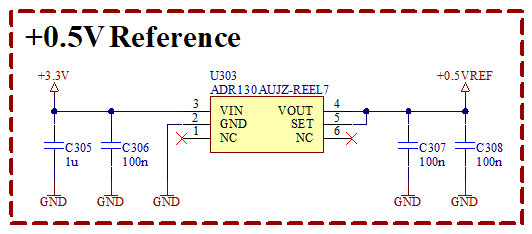
\includegraphics[width=10 cm]{Figures/BR_VREF.png}
    \caption{Referentni izvor napona od 0,5 V}
    \label{slk:BR_VREF}
\end{figure}

\subsection{Napajanje od 5 V}

Za napajanje od 5 V bilo je potrebno dizajnirati uzlazni prekidački regulator. Električna shema regulatora prikazana je na slici \ref{slk:BR_BOOST}. Odabran je TLV61220 proizvođača Texas Instruments jer je idealan za napajanje s baterije. Regulator može raditi na ulaznom naponu od 0,7 V do 5,5 V i potreban je mali broj vanjskih komponenti za rad \cite{ti:tlv61220}. Također je pogodan radi svoje male veličine u SOT-23 kućištu.
\begin{figure}[htb]
    \centering
    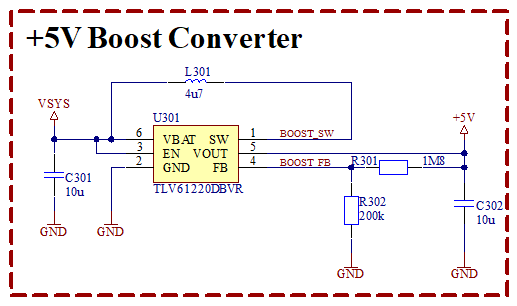
\includegraphics[width=10 cm]{Figures/BR_BOOST.png}
    \caption{Uzlazni prekidački regulator}
    \label{slk:BR_BOOST}
\end{figure}
Zavojnica je odabrana prema preporukama proizvođača, a naponsko djelilo je proračunato imajući na umu da donji otpornik ne bi trebao biti veći od $500\textrm{ k}\Omega$ kako bi vrijednost struje koja teče u FB stezaljku bila što bliže 0,01 $\mu\textrm{A}$ \cite{ti:tlv61220}. Efikasnost za izlazne struje od 1 mA do 50 mA je gotovo ista na ulaznom naponu u rasponu baterije i može se uzeti efikasnost od 90 \% (\ref{slk:BOOST_EFF}). Uz minimalni ulazni napon od 3 V, potrošnja, prema jednadžbi \ref{eq:IN_CURR} iznosi 75 mA.
\begin{figure}[H]
    \centering
    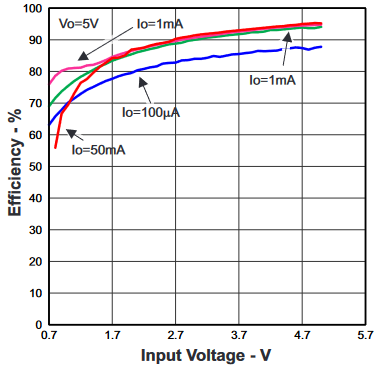
\includegraphics[width=6 cm]{Figures/BOOST_EFF.png}
    \caption{Efikasnost regulatora \cite{ti:tlv61220}}
    \label{slk:BOOST_EFF}
\end{figure}

\section{Baterija i punjač baterije}
\label{sec:BR_BATCHG}
Uzevši u obzir potrošnju svih podsustava ukupna struja koju punjač mora moći dati je ispod 430 mA. Uz struju punjenja baterije od 1 A i uzevši u obzir jednadžbe \ref{eq:IN_CURR} i \ref{eq:IN_CURR_MAX}, ukupna struja koju USB sučelje mora moći dati iznosi 1,08 A, što implicira da se može pretpostaviti ograničenje na ulaznu struju od 1,5 A. Uvjeti su slični onima kao kod središnjeg uređaja.

\subsection{Punjač baterije}
Električna shema punjača narukvice na slici \ref{slk:BR_BATCHG} slična je električnoj shemi sa slike \ref{slk:MB_BATCHG}. Promijenjena je svjetleća dioda za indikaciju punjenja u žutu, kako bi se jasnije mogla razlikovati indikacija između indikacije punjenja i indikacije statusa dobrog napajanja. Također su dodani veći otpornici u seriju s diodama jer je svjetlina bila prevelika.
\begin{figure}[H]
    \centering
    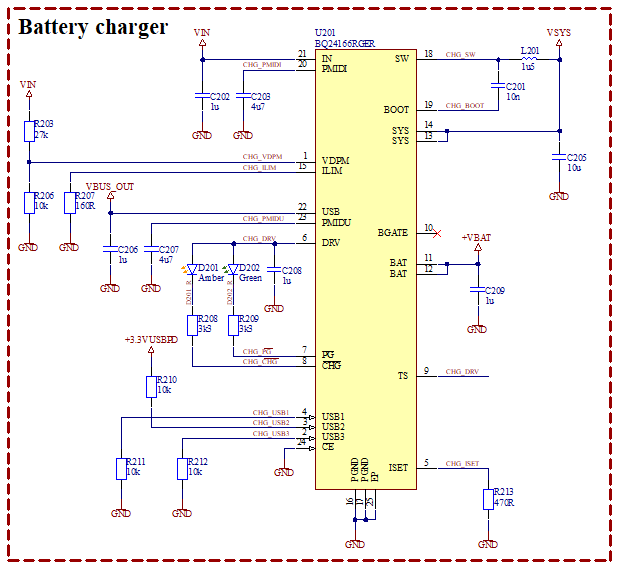
\includegraphics[width=0.95\textwidth]{Figures/BR_BATCHG.png}
    \caption{Električna shema punjača baterije na narukvici}
    \label{slk:BR_BATCHG}
\end{figure}

Još jedna razlika u odnosu na izvedbu na središnjem uređaju je u priteznim otpornicima na konfiguracijskim linijama za ograničenje struje USB-a, pri čemu je u slučaju ove pločice ograničenje postavljeno na 1,5 A zato jer nema potrebe za drugačijim postavkama i jer postoji ograničenje na veličinu pločice. S obzirom na ograničenje na dimenzije pločice, ovdje je odabrana zavojnica od 1,5 $\mu \textrm{H}$.

Posljednja razlika u odnosu na dizajn na središnjem uređaju je suptilna, ali ključna za ispravan rad punjača. Pogledom na električnu shemu na slici \ref{slk:MB_BATCHG} vidljivo je da stezaljka TS nije nigdje spojena, odnosno da se nalazi na plutajućem potencijalu. Ova stezaljka služi za mjerenje temperature baterije tijekom punjenja. Ako je temperatura prevelika ili premala, punjenje se zaustavlja. Električna shema mjerenja prikazana je na slici \ref{slk:BATCHG_TS}. Mjeri se napon na naponskom djelilu kojega čine otpornici i NTC termistor. Naponi na kojima se zaštita aktivira iznose 30\% i 60\% napona na stezaljci DRV, dakle 1,56 V i 3,12 V. S obzirom da je stezaljka TS plutajuća, napon na stezaljci je manji od donjega praga i punjenje ne radi. Kako bi se mjerenje temperature onemogućilo, napon na TS stezaljci mora biti veći od 70\% napona na stezaljci DRV. Iz tog razloga proizvođač preporučuje kratko spajanje stezaljki TS i DRV kako bi punjenje cijelo vrijeme bilo omogućeno.
\begin{figure}[htb]
    \centering
    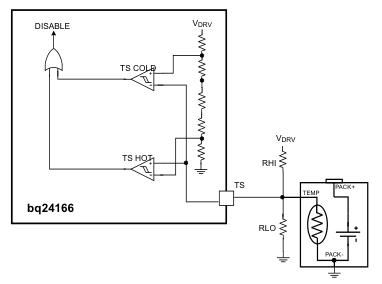
\includegraphics[width=10 cm]{Figures/BATCHG_TS.png}
    \caption{Mjerenje temprature senzora}
    \label{slk:BATCHG_TS}
\end{figure}

\subsection{Baterijska zaštita}
\sloppy Električna shema baterijske zaštite na narukvici je prikazana na slici \ref{slk:BR_BATPROT}. Shema je slična onoj sa središnjeg uređaja na slici \ref{slk:MB_BATPROT}, a ovdje su tranzistori pažljivije odabrani, sljedeći iskustva u testiranju prethodne implementacije sukladno preporukama proizvođača. Maksimalna struja pražnjenja iznosi prema \ref{sec:BR_BATCHG} iznosi 426,12 mA. Za aktivaciju zaštite pretpostavit će se struja od $I_{OCD}=1,5\textrm{ A}$, dakle otpor obaju FET-ova prema jednadžbi \ref{eq:TRANCUR} iznosi ${2R_{DS(on)}=66,67\textrm{ m}\Omega}$. Na temelju toga, struja na kojoj će se aktivirati zaštita za punjenje iznosi $I_{OCC}=1,5\textrm{ A}$. Dakle, tranzistor treba imati otpor $R_{DS(on)}=33,33\textrm{ m}\Omega$. Struja na kojoj će se aktivirati zaštita od kratkog spoja iznosi $I_{SCD}=7,5\textrm{ A}$, tako da tranzistor mora moći podnijeti tu struju. Prikaz promjene otpora u ovisnosti o naponu i struji odabranog tranzistora prikazana je na slici \ref{slk:RDS_NEW}. Vidljivo je da će otpor biti veći s većom strujom, što znači da će se zaštita aktivirati nešto prije vrijednosti proračunatih pragova, ali opet neće se aktivirati prerano da se onemogući punjenje, što je i poželjno s gledišta sigurnosti.
\begin{figure}[htb]
    \centering
    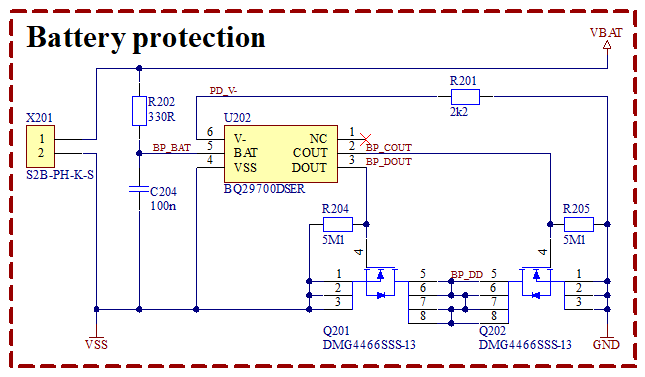
\includegraphics[width=10 cm]{Figures/BR_BATPROT.png}
    \caption{Baterijska zaštita na narukvici}
    \label{slk:BR_BATPROT}
\end{figure}
\begin{figure}[h!tb]
    \centering
    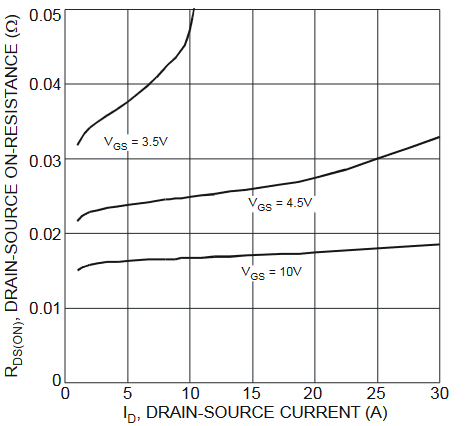
\includegraphics[width=6 cm]{Figures/RDS_NEW.PNG}
    \caption{Graf ovisnosti otpora o naponu između upravljačke elektrode i uvoda tranzistora DMG4466SSS-13 \cite{di:dmg4466}}
    \label{slk:RDS_NEW}
\end{figure}
S toga se može zaključiti da je ovo bolje projektirana zaštita u odnosu na onu na središnjem uređaju.

Ovdje su još dodani i otpori između upravljačke elektrode i uvoda tranzistora koji služe za bolje izbijanje naboja na kapacitetu između upravljačke elektrode i uvoda tranzistora \cite{ti:bq29700}.

\section{USB napajanje}
\label{sec:BR_USB}
Električna shema USB napajanja narukvice prikazana je na slici \ref{slk:BR_USB}. Dodan je pritezni otpornik R102 koji osigurava da ne dolazi do smanjenja napona na uvodu tranzistora Q101B radi diode u tranzistoru Q101A. Dodana je i Zener dioda od 10 V koja služi za zaštitu od prevelikog napona.

Osim toga, naponska djelila koja služe za podešavanje struje i napona USB-a se sada napajaju s internog regulatora čipa. Kod središnjeg uređaja (slika \ref{slk:MB_USB}) su se napajala s regulatora od 3,3 V koji se nalazi na pločici, što je u redu dokle god je priključena puna baterija. Međutim, u slučaju prazne ili isključene baterije dolazi do problema, jer je sada sustav ostao bez napajanja i ne mogu se podesiti naponi i struje USB-a. Ova uočena pogreška ispravljena je na opisani način, što je ujedno i preporuka proizvođača.
\begin{figure}[htb]
    \centering
    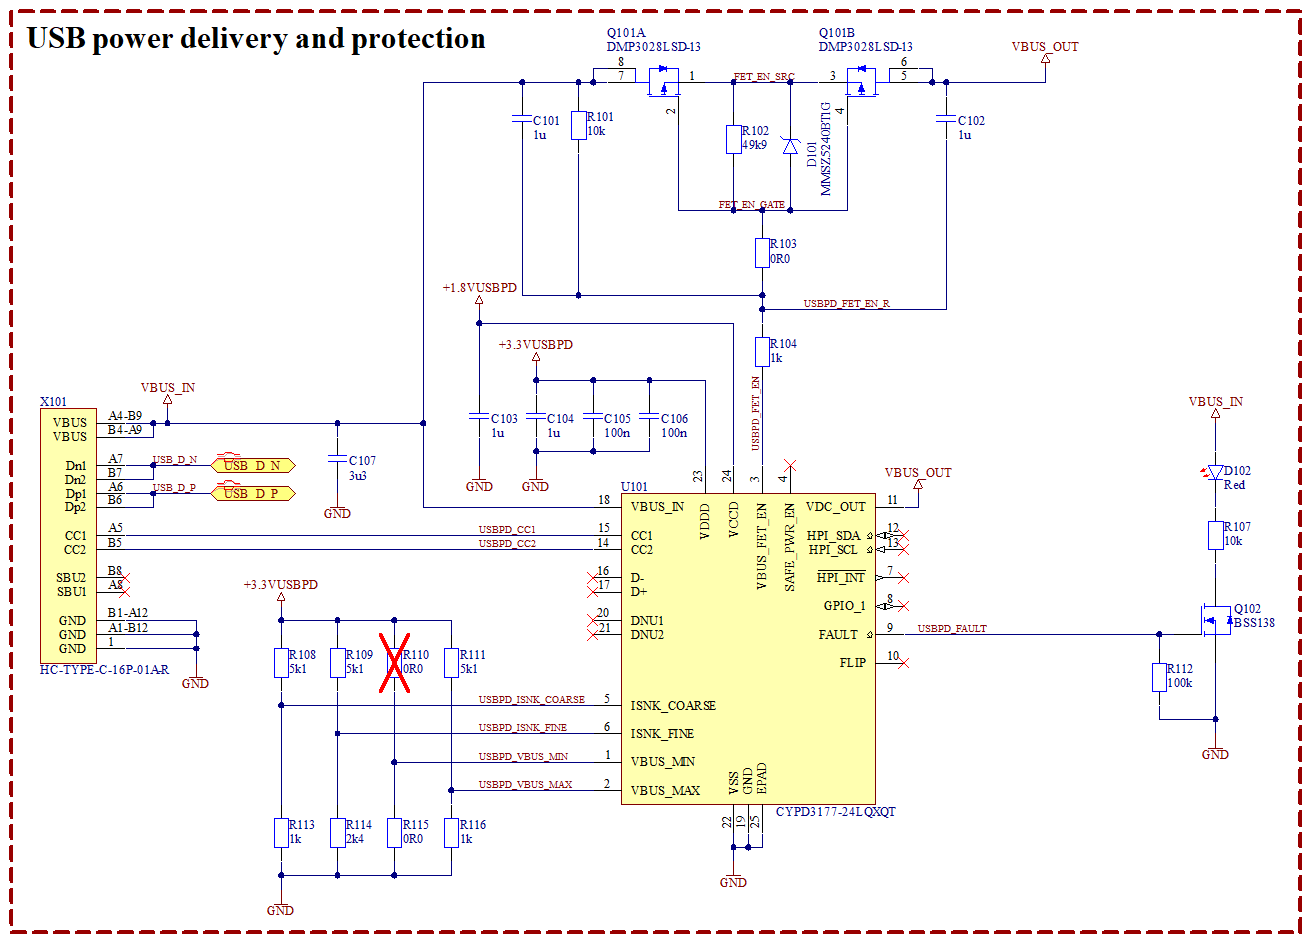
\includegraphics[width=\textwidth]{Figures/BR_USB.png}
    \caption{USB napajanje na narukvici}
    \label{slk:BR_USB}
\end{figure}
\section{Opis tiskane pločice}
Tijekom projektiranja tiskane pločice, osim što je bilo potrebno paziti na iste probleme kao i kod pločice središnjeg uređaja, bilo je potrebno voditi računa i na ograničenje prostora te na dvostranu montažu komponenti. Na slikama \ref{slk:BR_PCB_TOP} i \ref{slk:BR_PCB_BOT} prikazan je 3D prikaz projektirane pločice.

Za razliku od pločice središnjeg uređaja, ovdje je podsustav za bežičnu komunikaciju postavljen tako da se antena nalazi u potpunosti izvan pločice. Sukladno tome, podsustav za komunikaciju bolje će primati signale i stvarati manje smetnje na pločicu tijekom slanja signala.

Nadalje, bilo je potrebno ostvariti da se PPG senzor nalazi na dijelu narukvice koja ostvaruje kontakt s kožom pa je radi toga senzor smješten na donji sloj pločice (slika \ref{slk:BR_PCB_BOT}).

Radi ograničenja prostora uklonjene su sve ispitne točke i kratkospojnici.
\begin{figure}[htb]
    \centering
    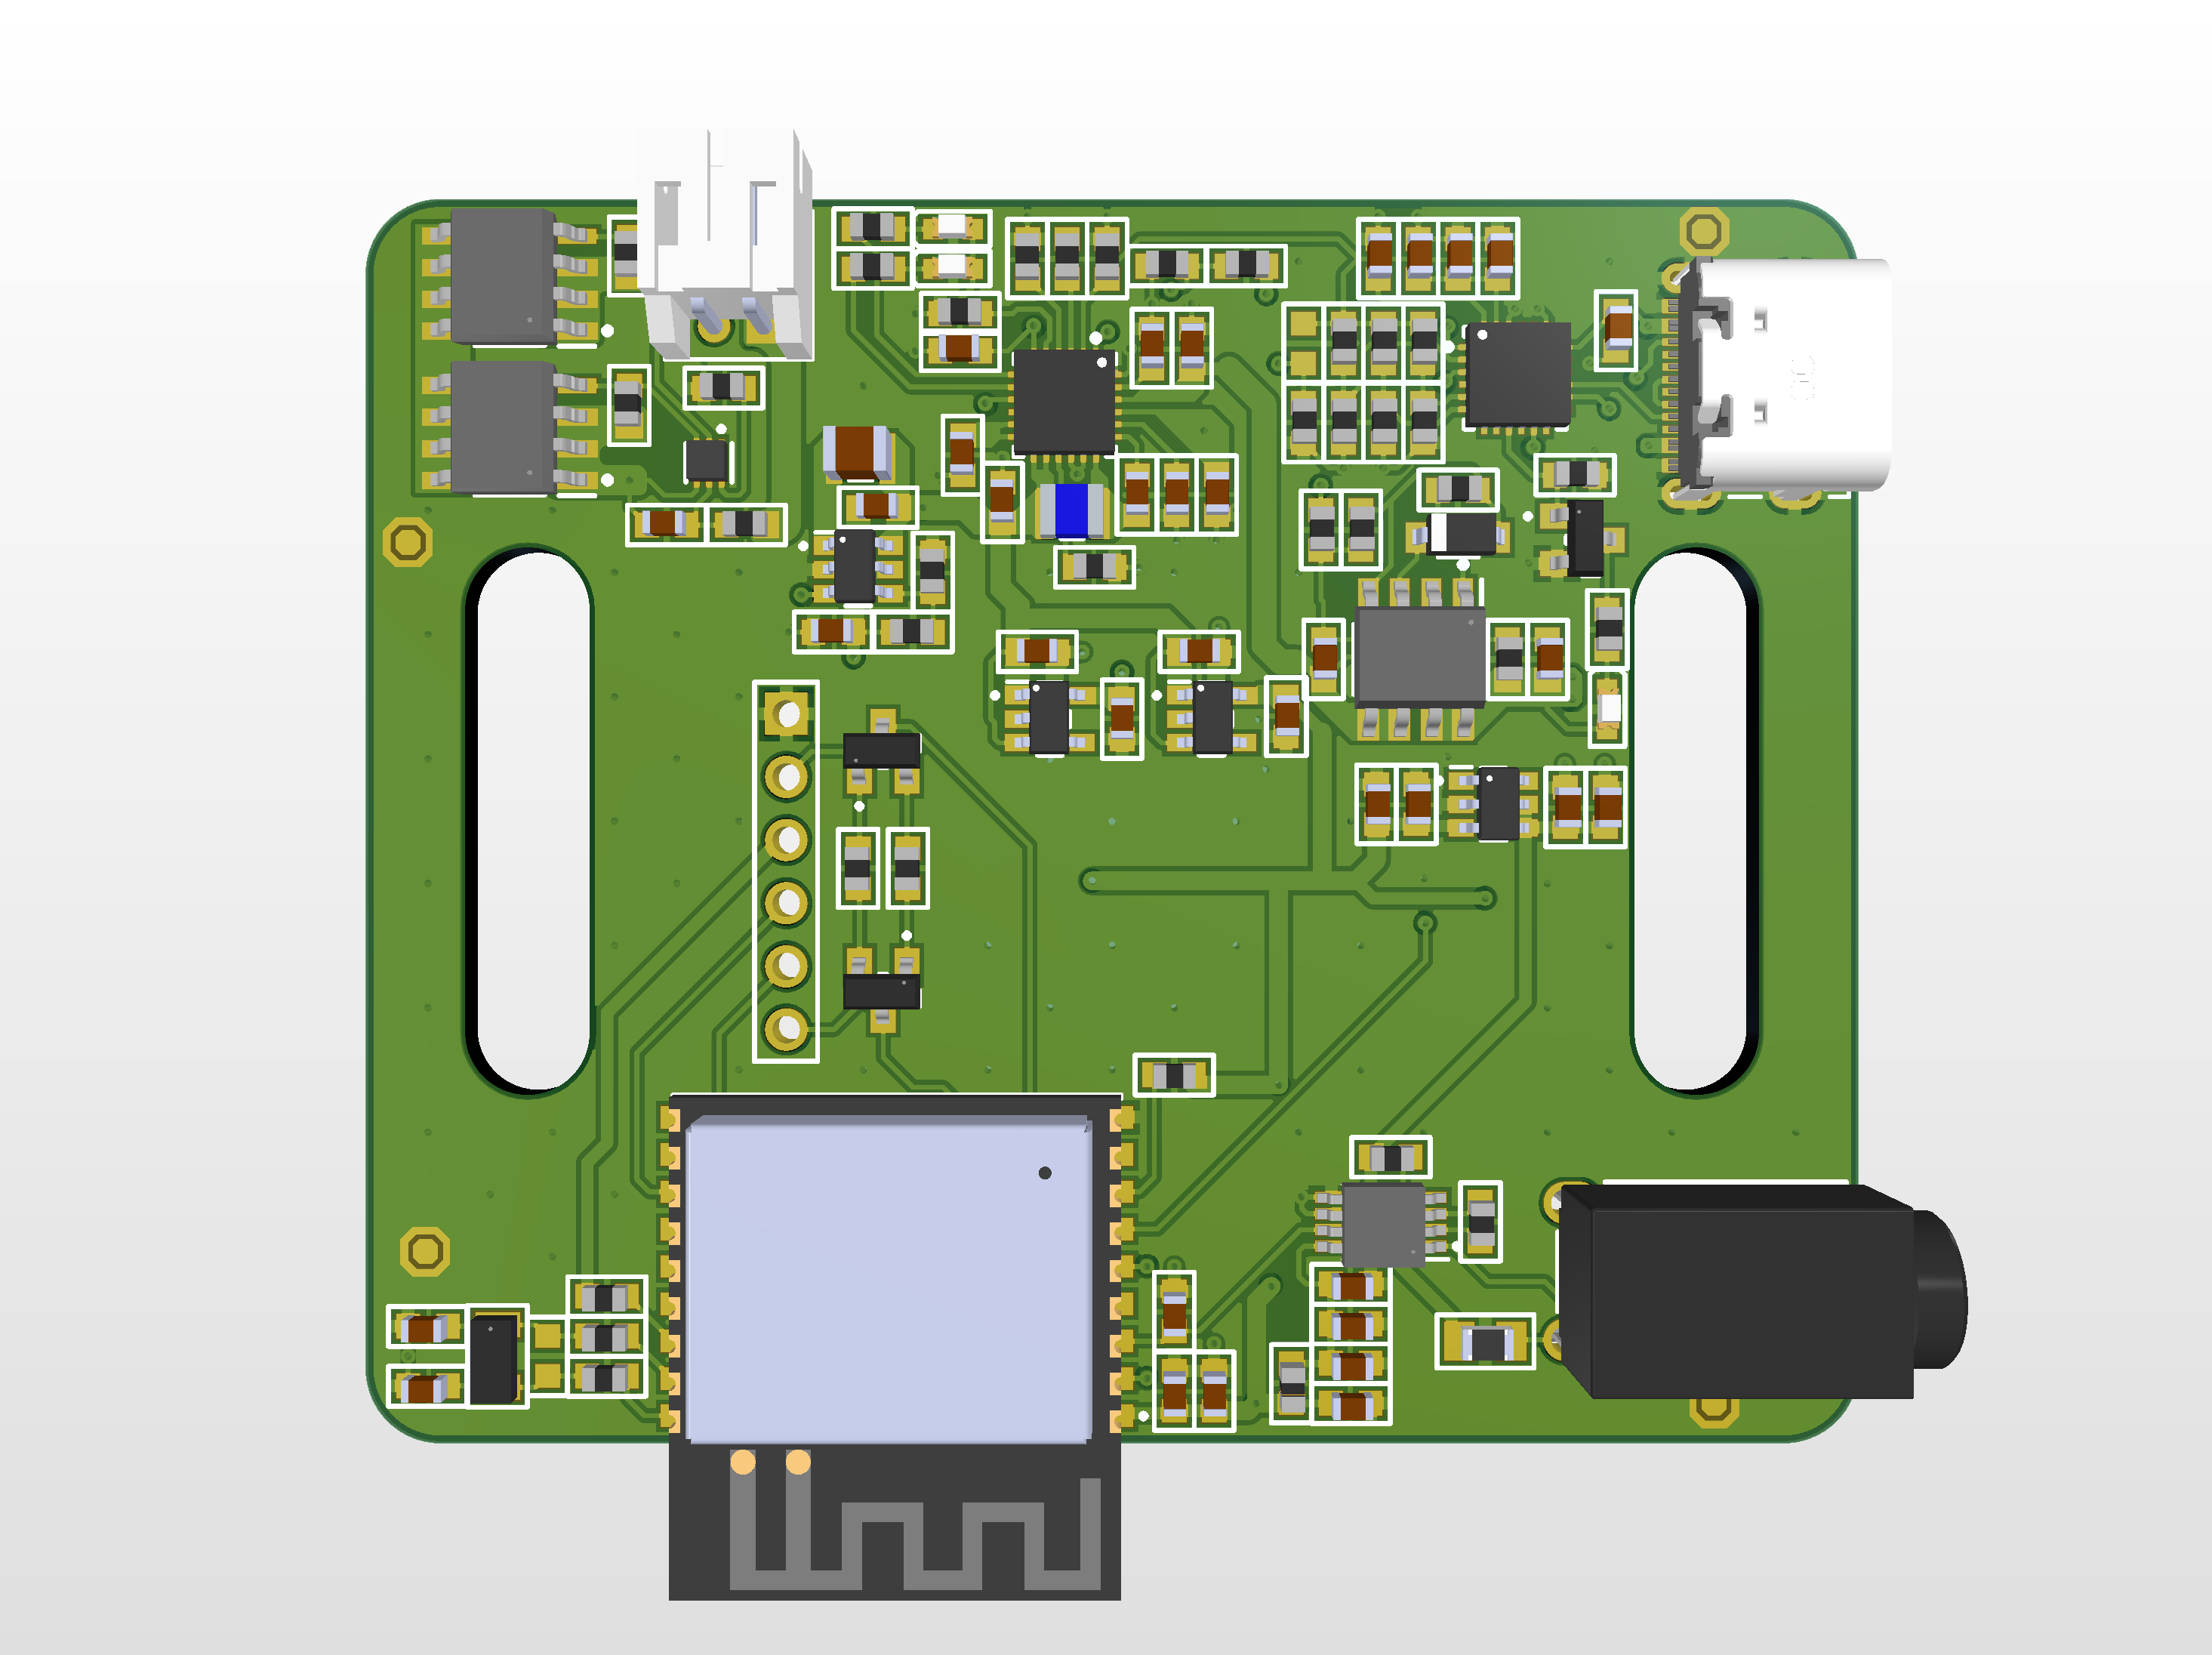
\includegraphics[width=10 cm]{Figures/BR_PCB.png}
    \caption{3D prikaz gornjeg sloja pločice}
    \label{slk:BR_PCB_TOP}
\end{figure}
\begin{figure}[htb]
    \centering
    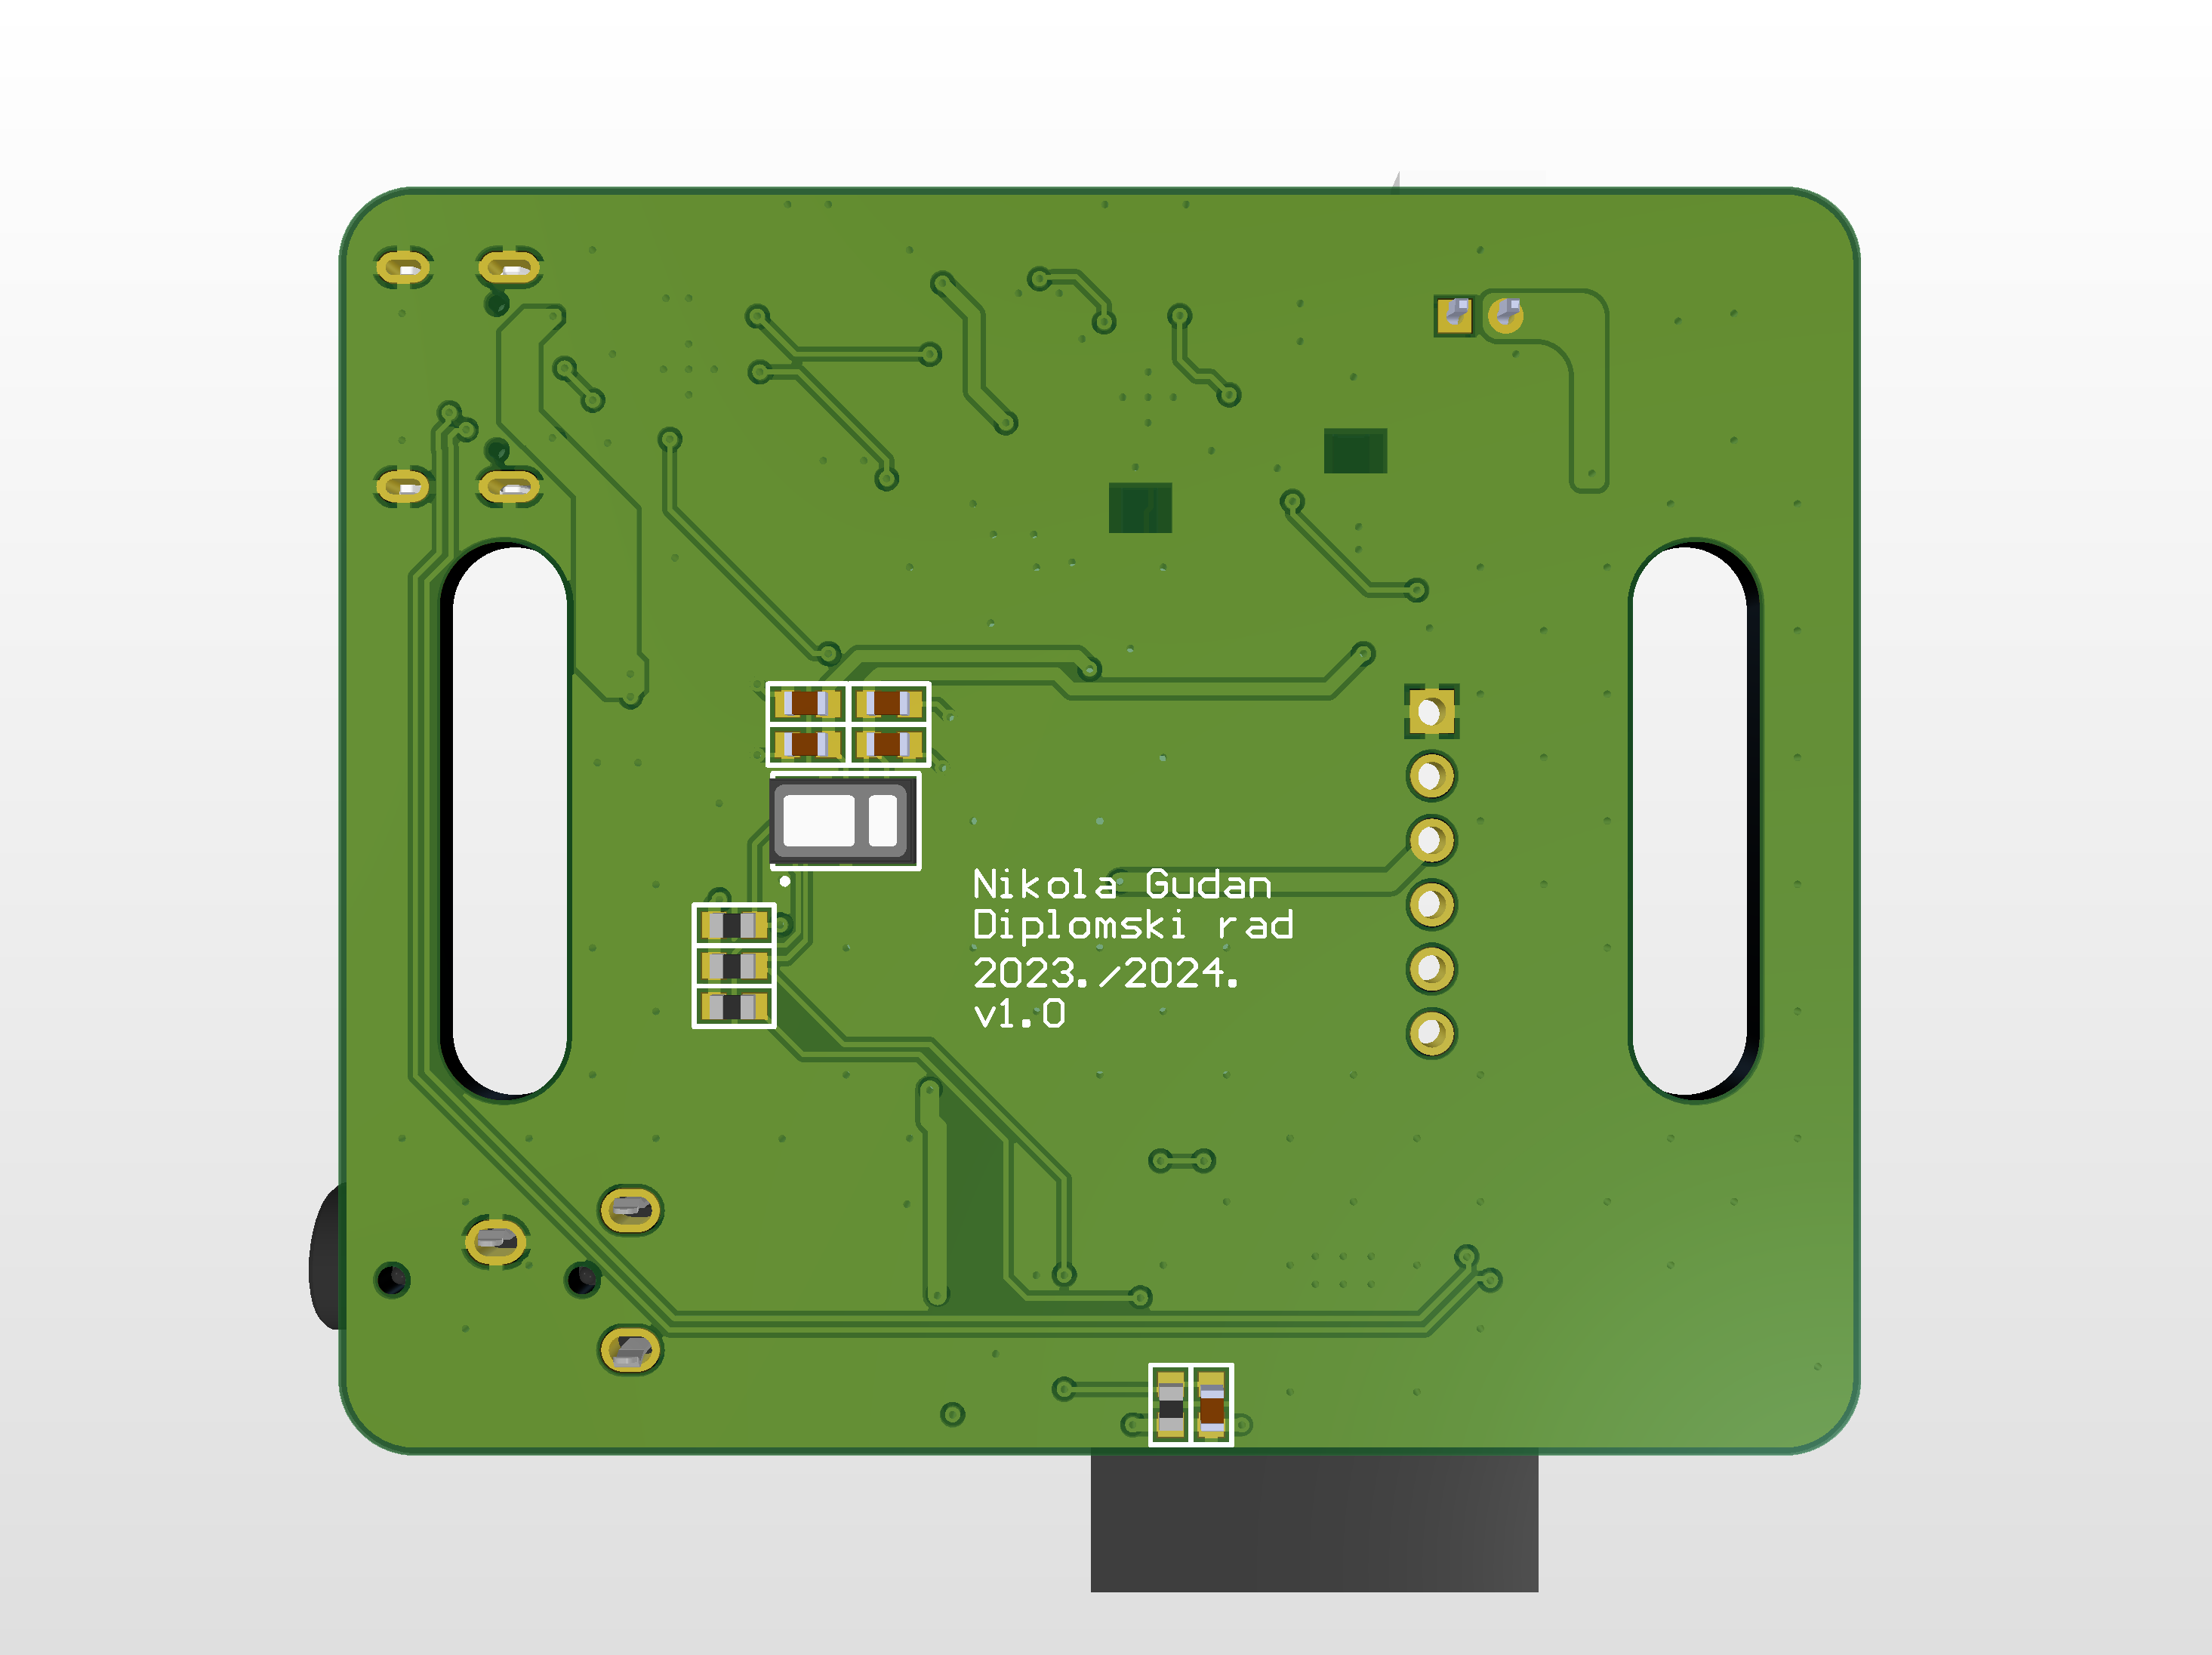
\includegraphics[width=10 cm]{Figures/BR_PCB_BOT.png}
    \caption{3D prikaz donjeg sloja pločice}
    \label{slk:BR_PCB_BOT}
\end{figure}